\RequirePackage{atbegshi}
\documentclass[compress]{beamer}
\usepackage[utf8]{inputenc}
\usepackage{pgfplots}
\usepackage[normalem]{ulem}
\useunder{\uline}{\ul}{}

\mode<presentation> {
   \usetheme{CambridgeUS}
 
   \usefonttheme[onlymath]{serif}
 
   \setbeamercovered{transparent}
}
\setbeamertemplate{navigation symbols}{}
\newcommand{\he}{\multicolumn} 

\title{An Analytical and Experimental Comparison of Sorting Algorithms}

\author{Adrian-Ioan Tuns}

\institute[Departament of computer science
Faculty of Mathematics and Informatics
West University of Timișoara] 
{Departament of computer science

Faculty of Mathematics and Informatics

West University of Timișoara}

\begin{document}


\frame{\titlepage}


\begin{frame}
\frametitle{Introduction}
\begin{itemize}
\item What does sorting algorithm mean?
\item Which algorithms are compared in this presentation?
\begin{itemize}
\item Insertion Sort
\item Quick Sort
\item Heap Sort
\end{itemize}
\item Complexity of algorithms
\item Special input cases of algorithms
\end{itemize}
\end{frame}


\begin{frame}
\frametitle{Insertion Sort}

\begin{columns}
\column{0.5\textwidth}
\begin{itemize}
\item What it is?
\item How it works?
\item Special cases
\item Complexity of $\mathcal{O}(n^2)$
\end{itemize}
\column{0.5\textwidth}

\begin{table}[]
\begin{tabular}{|l|l|l|l|l|}
\hline
8 & \textit{\textbf{3}} & 5 & 1 & 4 \\ \hline
3 & 8 & \textit{\textbf{5}} & 1 & 4 \\ \hline
3 & 5 & 8 & \textit{\textbf{1}} & 4 \\ \hline
1 & 3 & 5 & 8 & \textit{\textbf{4}} \\ \hline
1 & 3 & 4 & 5 & 8 \\ \hline
\end{tabular}
\end{table}

\end{columns}

\end{frame}

\begin{frame}
\frametitle{Quick Sort}

\begin{columns}
\column{0.5\textwidth}
\begin{itemize}
\item What it is?
\item How it works?
\item Special cases
\item Complexity of $\mathcal{O}(n\log{}n)$
\end{itemize}
\column{0.5\textwidth}

\begin{table}[]
\begin{tabular}{|l|l|l|l|l|}
\hline
3 & 2 & \textbf{5} & 4 & 1 \\ \hline
3 & \textbf{2} & \textit{1} & 4 & 5 \\ \hline
1 & 2 & \textbf{4} & \textit{3} & 5 \\ \hline
1 & 2 & 3 & 4 & 5 \\ \hline
\end{tabular}
\end{table}

\end{columns}

\end{frame}


\begin{frame}
\frametitle{Heap Sort}

\begin{columns}
\column{0.5\textwidth}
\begin{itemize}
\item What it is?
\item How it works?
\item Special cases
\item Complexity of $\mathcal{O}(n\log{}n)$
\end{itemize}
\column{0.5\textwidth}
\begin{table}[]
\begin{tabular}{|l|l|l|l|l|}
\hline
4 & 10 & 3 & 5 & 1 \\ \hline
\textbf{10} & 4 & \textit{3} & 5 & 1 \\ \hline
1 & 4 & 3 & \textit{5} & \textbf{10} \\ \hline
\textbf{5} & 4 & 3 & 1 & 10 \\ \hline
1 & 4 & 3 & \textbf{5} & \textbf{10} \\ \hline
\textbf{4} & 3 & 1 & \textbf{5} & \textbf{10} \\ \hline
1 & 3 & \textbf{4} & \textbf{5} & \textbf{10} \\ \hline
\end{tabular}
\end{table}
\end{columns}

\end{frame}

\begin{frame}
\frametitle{Input with ascending sorted numbers}

\begin{center}
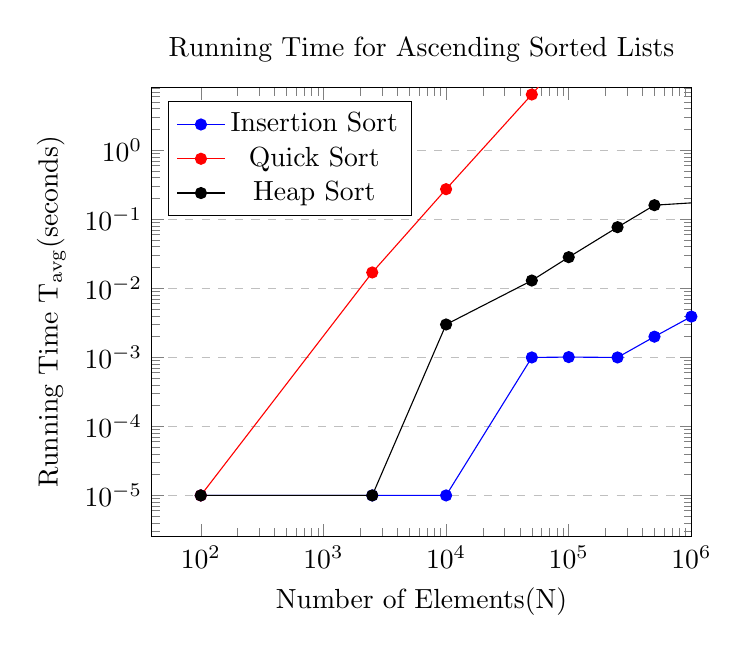
\begin{tikzpicture}
\centering
\begin{axis}[
   	title={Running Time for Ascending Sorted Lists},
    xlabel={Number of Elements(N)},
    ylabel={Running Time T\textsubscript{avg}(seconds)},
	xmode = log, ymode = log,    
    xmin=0, xmax=1000000,
    ymin=0, ymax=8,
    xtick={0,100,1000,10000,100000,1000000},
    ytick={},
    legend pos=north west,
    ymajorgrids=true,
    grid style=dashed,
]
 
\addplot[
    color=blue,
    mark=*,
    ]
    coordinates {
    (0,0)(100,0.00001)(2500,0.00001)(10000,0.00001)(50000,0.000997)(100000,0.001009)(250000,0.000997)(500000,0.001994)(1000000,0.0038986)
    };
 	\addlegendentry{Insertion Sort}
\addplot[
    color=red,
    mark=*,
    ]
    coordinates {
    (0,0)(100,0.00001)(2500,0.016966)(10000,0.272871)(50000,6.415868)(100000,26.449864)(250000,161.195339)(500000,608.42269)
    };
    \addlegendentry{Quick Sort}
 
\addplot[
    color=black,
    mark=*,
    ]
    coordinates {
    (0,0)(100,0.00001)(2500,0.00001)(10000,0.002993)(50000,0.012967)(100000,0.028249)(250000,0.076794)(500000,0.159903)(1000000000,0.374022)
    };
    \addlegendentry{Heap Sort}
    
\end{axis}
\end{tikzpicture}
\end{center}

\end{frame}

\begin{frame}
\frametitle{Input with descending sorted numbers}

\begin{center}
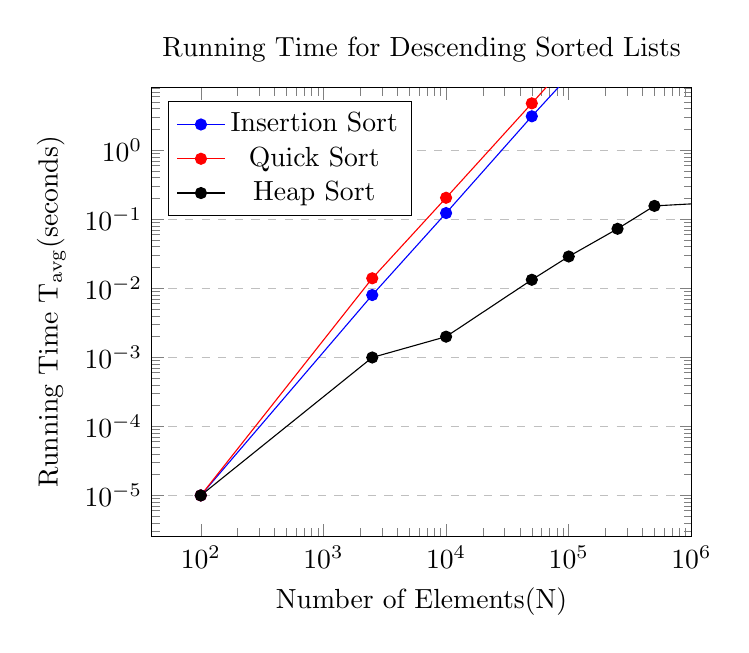
\begin{tikzpicture}
\centering
\begin{axis}[
   	title={Running Time for Descending Sorted Lists},
    xlabel={Number of Elements(N)},
    ylabel={Running Time T\textsubscript{avg}(seconds)},
	xmode = log, ymode = log,    
    xmin=0, xmax=1000000,
    ymin=0, ymax=8,
    xtick={0,100,1000,10000,100000,1000000},
    ytick={},
    legend pos=north west,
    ymajorgrids=true,
    grid style=dashed,
]
 
\addplot[
    color=blue,
    mark=*,
    ]
    coordinates {
    (0,0)(100,0.00001)(2500,0.007992)(10000,0.123008)(50000,3.099069)(100000,11.860596)(250000,73.638882)(500000,289.345398)(1000000,1134.02489)
    };
 	\addlegendentry{Insertion Sort}
\addplot[
    color=red,
    mark=*,
    ]
    coordinates {
    (0,0)(100,0.00001)(2500,0.013963)(10000,0.20481)(50000,4.775166)(100000,18.727545)(250000,115.963671)(500000,451.334676)
    };
    \addlegendentry{Quick Sort}
 
\addplot[
    color=black,
    mark=*,
    ]
    coordinates {
    (0,0)(100,0.00001)(2500,0.000996)(10000,0.001995)(50000,0.013297)(100000,0.028917)(250000,0.072809)(500000,0.156257)(1000000000,0.325122)
    };
    \addlegendentry{Heap Sort}
    
\end{axis}
\end{tikzpicture}
\end{center}

\end{frame}

\begin{frame}
\frametitle{Input with randomly generated numbers}

\begin{center}
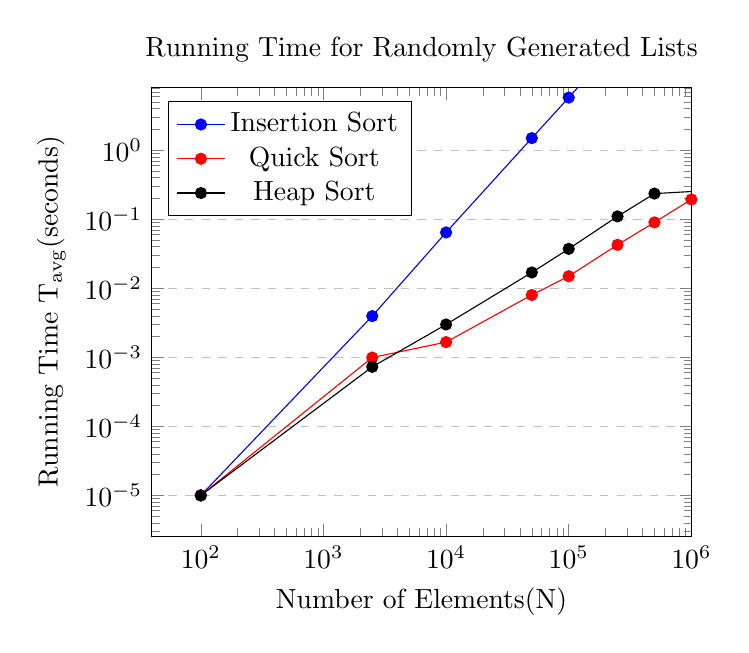
\begin{tikzpicture}
\centering
\begin{axis}[
   	title={Running Time for Randomly Generated Lists},
    xlabel={Number of Elements(N)},
    ylabel={Running Time T\textsubscript{avg}(seconds)},
	xmode = log, ymode = log,    
    xmin=0, xmax=1000000,
    ymin=0, ymax=8,
    xtick={0,100,1000,10000,100000,1000000},
    ytick={},
    legend pos=north west,
    ymajorgrids=true,
    grid style=dashed,
]
 
\addplot[
    color=blue,
    mark=*,
    ]
    coordinates {
    (0,0)(100,0.00001)(2500,0.003961)(10000,0.064499)(50000,1.497652)(100000,5.788853)(250000,35.427842)(500000,141.05064)(1000000,614.71654)
    };
 	\addlegendentry{Insertion Sort}
\addplot[
    color=red,
    mark=*,
    ]
    coordinates {
    (0,0)(100,0.00001)(2500,0.000994)(10000,0.001663)(50000,0.008012)(100000,0.014959)(250000,0.042656)(500000,0.090138)(1000000,0.19371)
    };
    \addlegendentry{Quick Sort}
 
\addplot[
    color=black,
    mark=*,
    ]
    coordinates {
    (0,0)(100,0.00001)(2500,0.000729)(10000,0.002992)(50000,0.016963)(100000,0.037242)(250000,0.110111)(500000,0.235308)(1000000000,0.507236)
    };
    \addlegendentry{Heap Sort}
    
\end{axis}
\end{tikzpicture}
\end{center}

\end{frame}

\begin{frame}
\frametitle{Questions}

\begin{center}
\Huge Questions?
\end{center}

\end{frame}

\end{document}